\documentclass[12pt]{article}
\usepackage[T1]{fontenc}
\usepackage{atbegshi}
\usepackage{graphicx}
\usepackage{hyperref}
\AtBeginDocument{\AtBeginShipoutNext{\AtBeginShipoutDiscard}}


\begin{document} \noindent
	\title{\Huge \textbf{Progetto Tecnologie Web}}
	\author{\textit{Preti Christian}}
	\date{2022}
	\maketitle 
	\noindent La relazione ha lo scopo di presentare il progetto svolto per il corso di \textit{Tecnologie Web}, ovvero un sito web per lo streaming di film e serie tv. \\ \\
	
	\noindent Saranno di seguito presentate le funzionalità principali del sito: \\
	\begin{itemize}
		\item Possibilità di recensire un film, con 1 $\sim$ 5 stelle e commento scritto.
		\item Panoramica delle recensioni scritte da un determinato utente.
		\item Lista di tutte le recensioni di un determinato film, con valutazione media.
		\item Ranking dei film in base alla valutazione media.
		\item Possibilità di cercare film in base al genere o con un voto minimo/massimo.
		\item Inserire un film tra i preferiti.
		\item Recommendation system operante sui generi preferiti di un utente, basandosi sulle recensioni di altri utenti a film guardati da entrambi.
		\item Chat di gruppo relativa ad un determinato film. \\
	\end{itemize}
	
	\noindent Nella prossima pagina verranno dati qualche approfondimenti su alcune di queste. 
	\pagebreak
	
	
	
	\noindent \centerline {\Huge \textbf{Approfondimenti sulle funzionalità}} \\ \\
	
	\noindent \textbf{Home}: Essa contiene i form di login/registrazione. E' possibile anche accedere al sito come utenti anonimi, attraverso il tasto '\textit{Entra come guest}'. \\
	
	\noindent \textbf{Ranking}: I parametri su cui è possibile fare ranking sono:
	\begin{itemize}
		\item Titolo.
		\item Valutazione, sia essa minima che massima.
		\item Genere. \\
	\end{itemize}

	\noindent \textbf{Recommendation System}: 
	
	\noindent \textbf{Chat}: Rappresentata come una semplice pagina in cui gli utenti, dopo aver necessariamente guardato il film, avranno modo di commentarlo con altri utenti.
	
	\pagebreak
	
	
	\noindent \centerline {\Huge \textbf{Tecnologie utilizzate}} \\ \\
	
	\noindent \textbf{Frontend}: Le tecnologie utilizzate lato frontend sono state: 
	\begin{itemize}
		\item \textbf{Bootstrap}: E' probabilmente il framework più utilizzato in ambito frontend, in grado di ricoprire i vari HTML, CSS e JavaScript. Ho fatto largo uso di Bootstrap, al fine di disegnare in modo facile e veloce le varie pagine del sito. \\
		
		\item \textbf{Chart.js}: E' una libreria che permette di importare grafici all'interno del proprio sito. È molto ben fatta, ben documentata e facile da usare. In questo contesto, è stata usata per disegnare un \textit{grafico poligonale} all'interno della pagina di account dell'utente. \\
	\end{itemize}

	\noindent Lato \textbf{Backend}, invece: 
	\begin{itemize}
		\item \textbf{SQLite}, data la comodità nel gestire il database in modo single-file e per la sua diretta integrazione con Django. \\
		
		\item \textbf{VSCode}, data la comodità nell'avere plugin che renderizzassero live le pagine HTML durante la scrittura, cosa che ha velocizzato molto il workflow. Inoltre, i plugin per la gestione dei test, facilmente avviabili in qualsiasi momento. Oltretutto, la possibilità di passare facilmente da un linguaggio di markup quale HTML o CSS, a Python/JavaScript.
	\end{itemize}
	\pagebreak

	
	\noindent \centerline {\Huge \textbf{Divisione nelle varie app}} \\ \\ 
	Il progetto è stato diviso in 4 app:
	
	\begin{itemize}
		\item \textbf{Streamify}: È l'app principale del progetto, essa contiene le varie pagine, come ad esempio l'homepage, il catalogo dei film, la pagina \textit{'Il mio account'}. 
		
		\item \textbf{Chatify}: Come suggerisce il nome, essa fornisce il servizio di chat all'interno del sito. Ho deciso di separarla da Streamify, al fine di vederlo come un \textit{'servizio ausiliario'}, un po' come se fosse una feature esterna rispetto allo scopo \textit{principale} del sito.
		
		\item \textbf{Auth}: Anche l'autenticazione è stata separata dal sito principale, dato che ho cercato di tenere le varie logiche quanto più separate possibili, al fine di aumentare la modularità del sito e la sua portabilità.
		
		\item \textbf{TestApp}: Essa contiene i test di tutte le app citate sopra, creando un'app dedicata a questo scopo, mi è stato più facile gestirli, potendoli raggruppare tutti sotto la stessa directory. Ulteriori dettagli su questo verranno affrontati nel paragrafo dedicato.
	\end{itemize}
	\pagebreak
	
	
	\noindent \centerline {\Huge \textbf{Ulteriori dettagli sulle funzionalità/scelte adottate}} \\ \\
	
	\noindent \textbf{Recommendation System}: Esso è stato pensato come la somiglianza tra la doppia \{genere: voto medio\} di ogni utente verso ogni genere presente nel database.
	Inoltre, verranno dati suggerimenti solamente sui due generi preferiti da utente, dato che difficilmente egli vorrà ricevere consigli su generi che non gli interessano. \\Questa lista di due generi \textit{preferiti} verrà calcolata per ogni utente e verranno cercate delle corrispondenze tra gli elementi. Se trovati, si guarderà la differenza di voto medio al genere. Più la differenza sarà bassa, più si può presumere che i gusti, quantomeno su quel genere, tra i due utenti siano simili, e verranno consigliati all'utente loggato quelli guardati dall'altro utente, ma non da lui. \\
	Poniamo ad esempio:
	\begin{verbatim}
		U1: {
		'Azione': 4.5,
		'Avventura': 4.8,
	}

	U2: {
		'Azione': 4.4,
		'Avventura': 5.0,
	}
	\end{verbatim}

	\noindent Ipotizzando che i due generi preferiti dei due utenti siano quelle sopra citate, verrà trovato un match per entrambi i generi, dato che entrambi i generi di U1 sono i preferiti anche di U2, a questo punto bisogna calcolare la similarità, ovvero \textbf{quanto} il suggerimento può essere inerente, la formula sarà: \\
	
	$100 - {100 * |VotoGenereU1-VotoGenereU2| \over 5}$ \\ \\
	
	\noindent In questo esempio, all'utente U1 verranno suggeriti con una precisione del 98\% i film di genere \textit{Azione} guardati da U2 (ma ovviamente non da U1) e allo stesso modo con la precisione del 96\% i film di genere \textit{Avventura}. \\
	
	
	
	\noindent \textbf{Gestione delle sessioni}: L'utente loggato è stato gestito attraverso l'uso di \textbf{session}, ovvero un dizionario Python facente parte del parametro \textit{request}, in cui è possibile salvare valori relativi alla sessione corrente.
	Le sessioni possono poi essere personalizzate in base alle proprie preferenze attraverso vari parametri, personalmente ho fatto uso dei seguenti, impostati nel file \textit{settings.py}:
	\begin{verbatim}
		SESSION_EXPIRE_AT_BROWSER_CLOSE = True
		SESSION_COOKIE_AGE = 180
	\end{verbatim}
	
	\noindent Con \textit{age} si intende la durata della validità, in secondi, della sessione, prima che il sito chieda di nuovo all'utente di effettuare l'accesso. \\ \\
	
	\noindent \textbf{Tipi di utenti}: Gli utenti, all'interno del sito, sono di 3 tipi:
	\begin{itemize}
		\item \textbf{Anonimo}: L'utente \textit{anonimo} è un utente coi permessi di base. Gli è concesso entrare nel catalogo attraverso il pulsante \textit{Entra come guest}, può solamente sfogliare il catalogo dei film e consultarne i dettagli, come titolo, valutazione media, anno di uscita...
		 
		\item \textbf{Loggato}: Un utente \textit{loggato} ha invece la possibilità di guardare un film, attraverso un pulsante presente difianco al film, nel catalogo. Ha la possibilità di consultare la propria pagina \textit{Il mio account}, per avere la lista dei film da egli guardati, le recensioni lasciate e i film suggeriti dal recommendation system. Sempre in questa pagina è presente anche il grafico reso disponibile da Chart.js, che mostra in modo user-friendly i generi preferiti.
		\item \textbf{Admin}: L'utente \textit{admin} è inteso come l'amministratore/gestore del sito. Ha il permesso di aggiungere, modificare ed eliminare utenti, film e generi. 
		
		\item \textbf{Template tags}: Un template tag è una sorta di funzione applicabile ad un template. Nel mio caso ne ho implementata solamente una, chiamata \textit{replace\_titles}, la sua funzione è quella di prendere in input il titolo di un film, che avrà dei \_ al posto dei whitespace (per comodità nei link, quando passato come parametro GET), e sostituirà quest'ultimi con dei whitespace appropriati, si tratta quindi solamente di un workaround \textit{grafico}.
	\end{itemize}
	\pagebreak
	
	
	
	\noindent \centerline {\Huge \textbf{Modelli}} \\
	
	\noindent All'interno del progetto sono presenti 4 entità:
	
	\begin{itemize}
		\item \textbf{Utente}: Un \textit{utente} è definito dai seguenti \textit{fields}:
		\begin{itemize}
			\item \textbf{username}
			\item \textbf{email}
			\item \textbf{password}
			\item \textbf{nome}
			\item \textbf{cognome} \\
		\end{itemize}
		
		\item \textbf{Film}:
		\begin{itemize}
			\item \textbf{titolo}
			\item \textbf{generi}
			\item \textbf{anno\_uscita}
			\item \textbf{trama} \\
		\end{itemize}
		
		
		\item \textbf{Genere}:
		\begin{itemize}
			\item \textbf{name}: Rappresenta il nome del genere, e.g \textit{Azione, avventura...} \\
		\end{itemize}
		
		
		
		\item \textbf{Recensione}:
		\begin{itemize}
			\item \textbf{voto}: Rappresenta il voto numerico della recensione, con range 1$\sim$5.
			\item \textbf{film}: \textit{Foreign Key} che specifica il film recensito.
			\item \textbf{utente}: \textit{Foreign Key} che specifica l'utente autore della recensione.
			\item \textbf{commento\_scritto}: Commento scritto opzionale.
		\end{itemize}
	\end{itemize}
	\pagebreak
	
	
	\noindent \centerline {\Huge \textbf{Testing}} \\
	
	\noindent Come specifica nel paragrafo riguardo alla divisione in app, i test sono stati separati dal resto delle applicazioni, questo ha permesso di facilitare la loro gestione, permettendomi di raggrupparli tutti sotto la stessa app. Dentro il path ./test\_apps/tests, possiamo trovare varie directory. \\Ho deciso di separare anche qui i test al fine di tenerli ordinati e poter, su richiesta, eseguire test riguardanti un preciso/solo alcuni argomenti. \\
	Per i test mi sono affidato a \textit{Django Unit Test Framework}, che sfrutta nativamente \textit{unittest}.
	I test totali sono 33. \\
	Sono presenti più test per ogni singola view, dato che è stato testato ogni possibile aspetto di ogni view, ovvero il caso di \textit{success}, \textit{fail} e \textit{conflict}. \\ \\
	Per orientarmi durante la scrittura di un test, è stato utile assegnare lo status code manualmente ad ogni render delle view:
	\begin{itemize}
		\item Se l'utente effettua l'accesso con successo, lo status code sarà 200 (\textbf{Successo}).
		\item Se l'utente inserisce credenziali errate, lo status code sarà 401 (\textbf{Unauthorized}).
		\item Se l'utente si registra con username o email già in uso, lo status code sarà 409 (\textbf{Conflitto}).
	\end{itemize}
	\pagebreak
	
	
	\noindent \centerline {\Huge \textbf{Schemi}} \\ \\ \\
	\centering 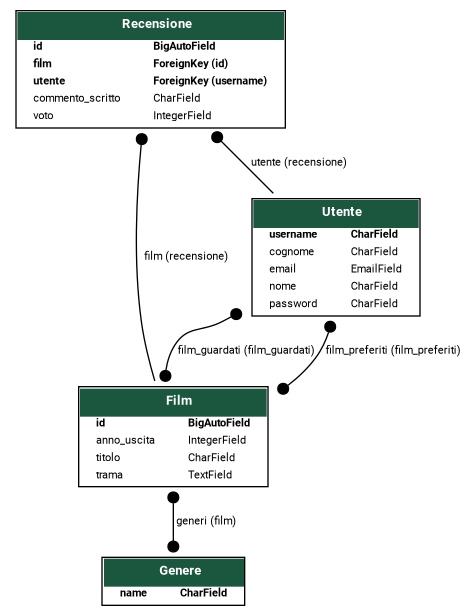
\includegraphics[width=11cm, ]{Immagini/uml_schema_streamify.png} \\
	\centering Schema UML
	
	
	
	

\end{document}